\documentclass{article}

\usepackage{graphicx}
\usepackage{tikz}
\usepackage{tikzsymbols}
\usetikzlibrary{calc,patterns,shapes.geometric}
\pagestyle{empty}
\usepackage[margin=0pt]{geometry}
\geometry{papersize={14in,12in}}

\def\centerarc[#1](#2)(#3:#4:#5){\draw[#1] ($(#2)+({#5*cos(#3)},{#5*sin(#3)})$) arc (#3:#4:#5);}

\begin{document}
	\begin{figure}
		\centering
		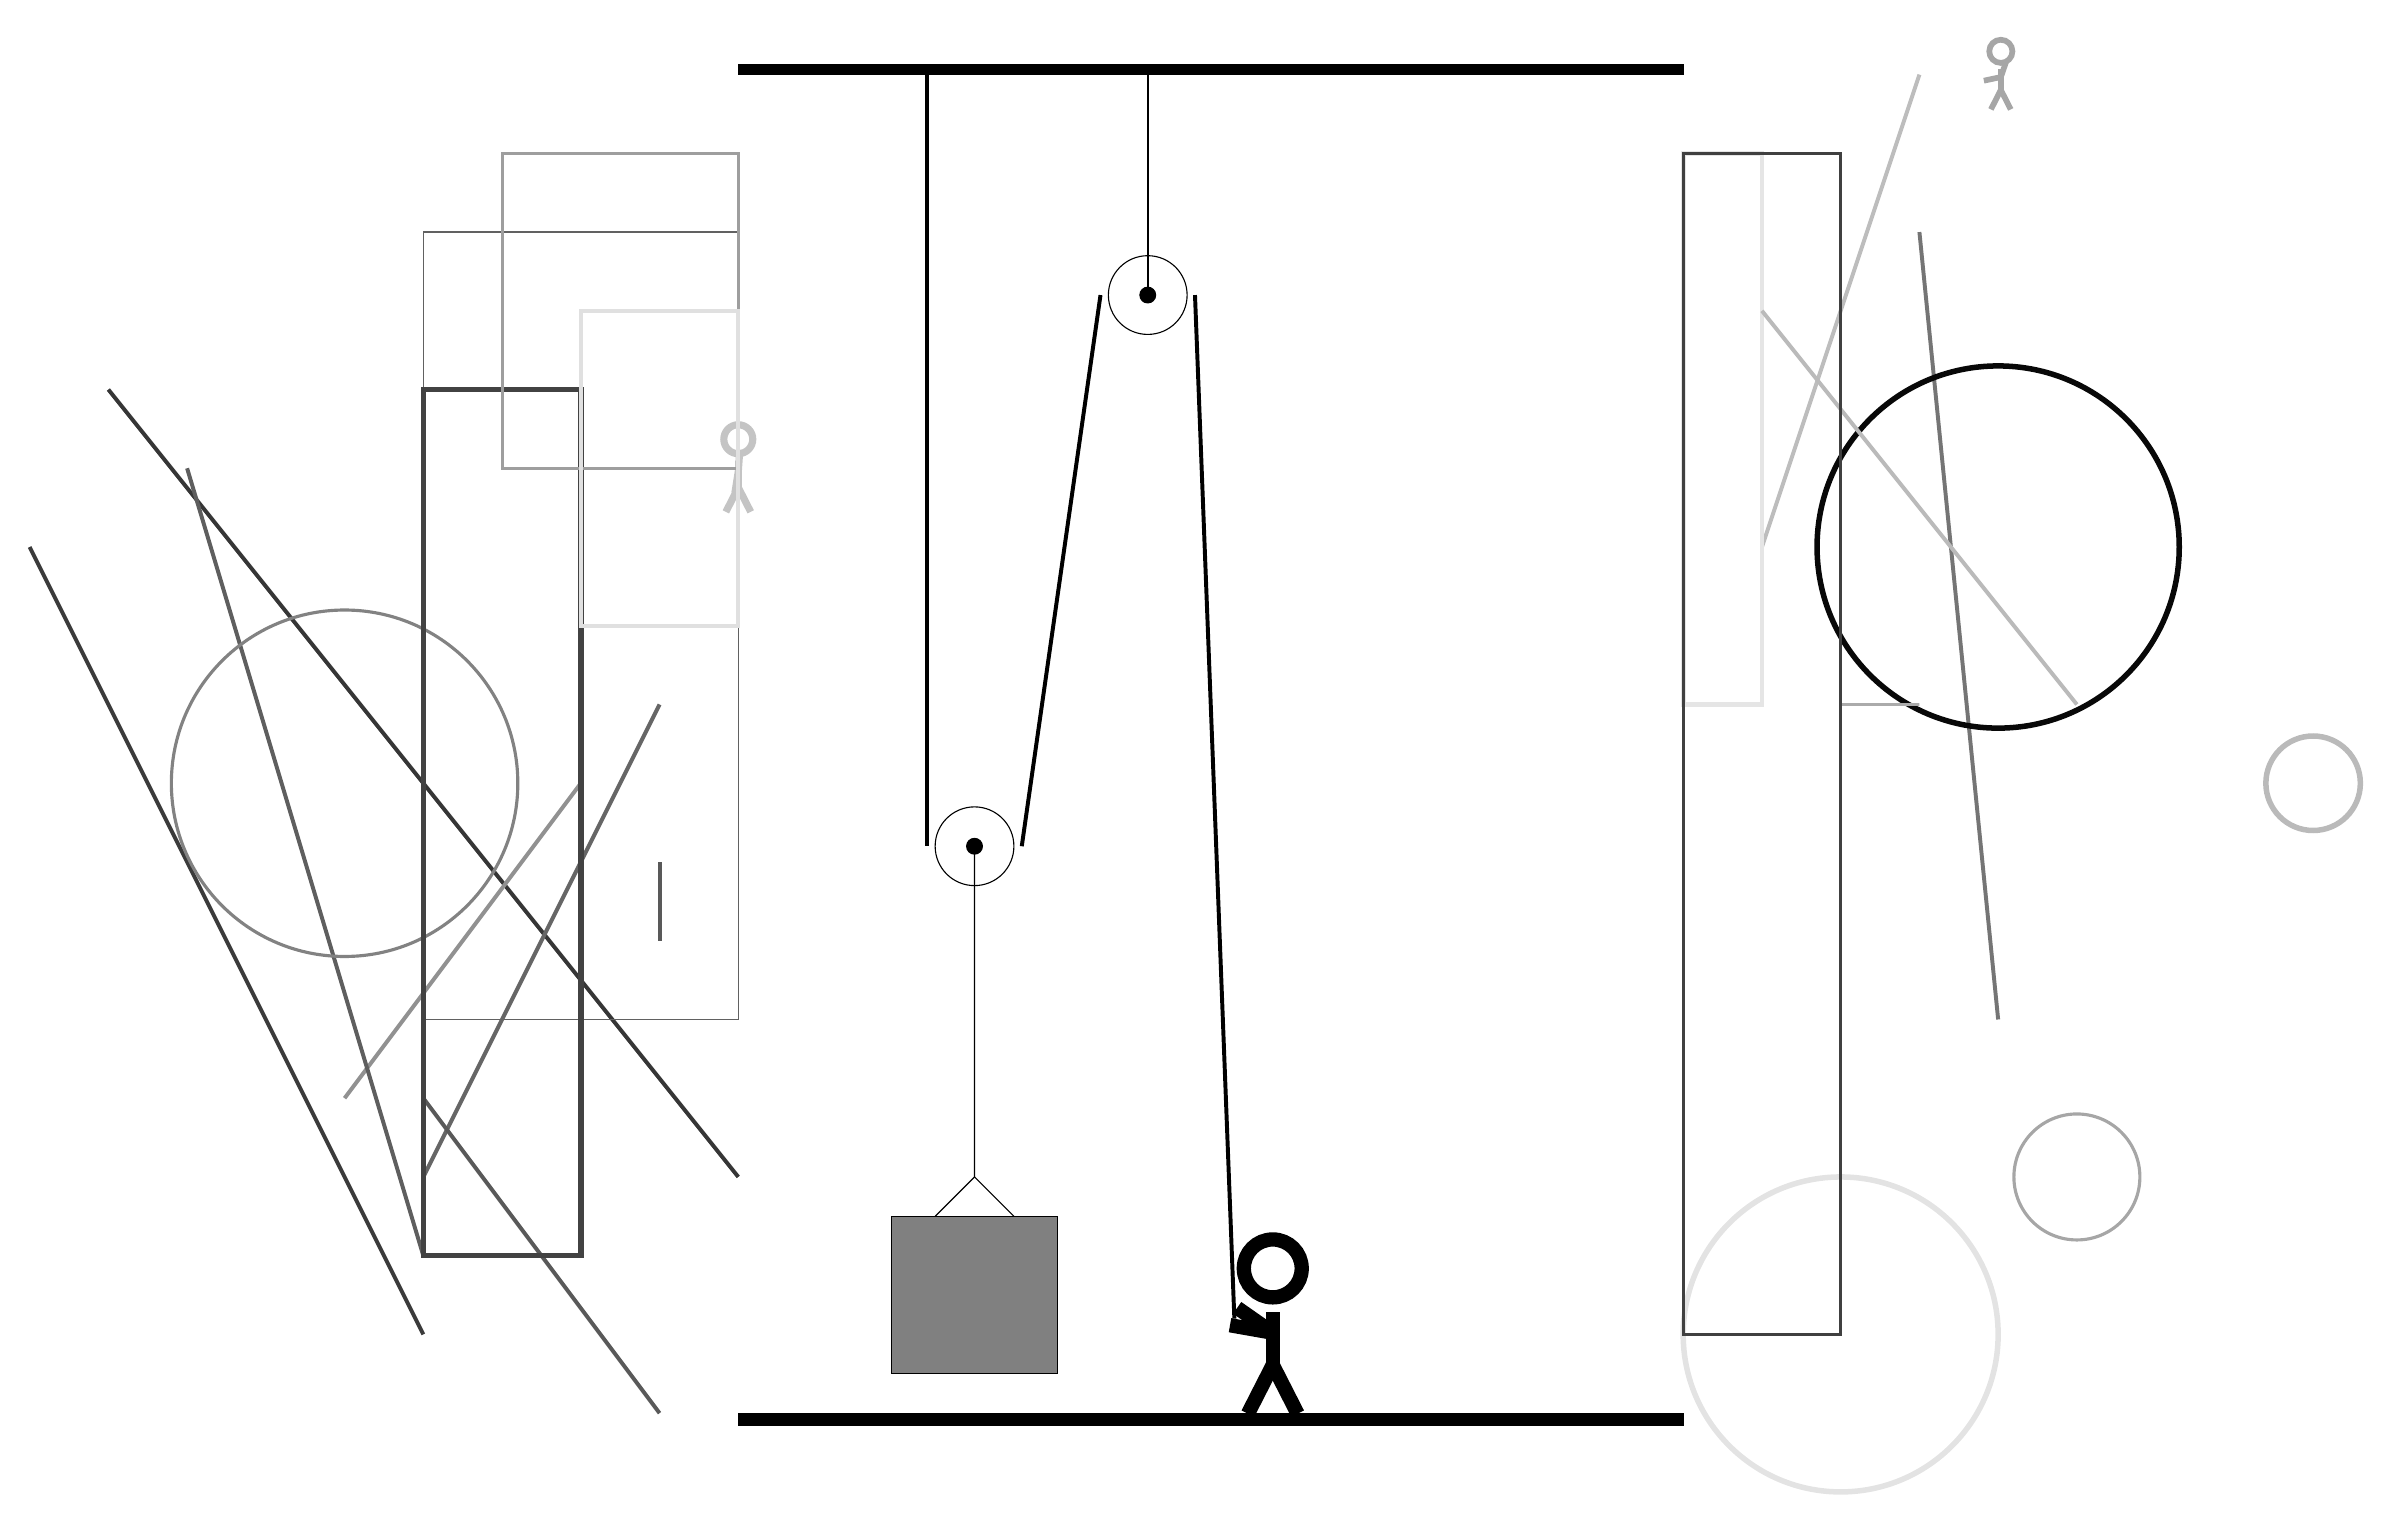
\begin{tikzpicture}
			%%%%% START %%%%%
			
			\draw[fill=black] (-2, 14) rectangle (10, 14.125);
			
			\draw [line width=0.7mm, color=black!11](12, -2) circle (2.0);
			
			\draw[line width=0.5mm, color=black!79](-2, 0) -- (-10, 10);
			\draw[line width=0.2mm, color=black!62] (-2, 12) rectangle (-6, 2);
			\node[line width=0.5mm, color=black!35] at (14, 14) {\Strichmaxerl[4][12][71]};
			\draw [line width=0.7mm, color=black!27](18, 5) circle (0.6);
			\draw[line width=0.5mm, color=black!60](-6, 0) -- (-3, 6);
			\draw [line width=0.4mm, color=black!35](15, 0) circle (0.8);
			
			\draw[line width=0.5mm, color=black!54](13, 12) -- (14, 2);
			\draw [line width=0.7mm, color=black!97](14, 8) circle (2.3);
			\draw[line width=0.5mm, color=black!77](-6, -2) -- (-11, 8);
			\node[line width=0.2mm, color=black!23] at (-2, 9) {\Strichmaxerl[5][81][86]};
			
			\draw[line width=0.3mm, color=black!33] (12, 6) rectangle (13, 6);
			\draw[line width=0.5mm, color=black!43](-7, 1) -- (-4, 5);
			
			\draw[line width=0.5mm, color=black!26](11, 8) -- (13, 14);
			\draw[line width=0.6mm, color=black!10] (11, 6) rectangle (10, 13);
			\draw[line width=0.5mm, color=black!63](-6, -1) -- (-9, 9);
			
			\draw[line width=0.5mm, color=black!52] (-4, 11) rectangle (-3, 11);
			
			\draw[line width=0.5mm, color=black!65](-3, -3) -- (-6, 1);
			\draw[line width=0.5mm, color=black!27](15, 6) -- (11, 11);
			\draw [line width=0.4mm, color=black!49](-7, 5) circle (2.2);
			\draw[line width=0.7mm, color=black!74] (-4, 10) rectangle (-6, -1);
			
			\draw[line width=0.4mm, color=black!10] (12, 12) rectangle (12, -2);
			
			\draw[line width=0.4mm, color=black!38] (-2, 13) rectangle (-5, 9);
			\draw[line width=0.5mm, color=black!12] (-4, 11) rectangle (-2, 7);
			\draw[line width=0.5mm, color=black!65](-3, 3) -- (-3, 4);
			
			\draw[line width=0.4mm, color=black!75] (10, -2) rectangle (12, 13);
			
			\draw (3.2, 11.2) circle (0.5);
			\draw[fill=black] (3.2, 11.2) circle (0.1);
			\draw[thick] (3.2, 11.2) -- (3.2, 14);
			
			\draw (1, 4.2) circle (0.5);
			\draw[fill=black] (1, 4.2) circle (0.1);
			
			\draw (1, 4.2) -- (1, 0) -- (0.5, -0.5);
			\draw (1, 0) -- (1.5, -0.5);
			\draw[fill=black!50] (-0.05, -0.5) rectangle (2.05, -2.5);
			
			\draw[line width=0.5mm] (0.4, 14) -- (0.4, 4.2);
			\centerarc[line width=0.5mm](1, 4.2)(180:360:0.6);
			\draw[line width=0.5mm](1.6, 4.2) -- (2.6, 11.2);
			\centerarc[line width=0.5mm](3.2, 11.2)(0:180:0.6);
			\draw[line width=0.5mm](3.8, 11.2) -- (4.3, -1.8);
			
			\node at (4.7, -1.9) {\Strichmaxerl[10][-35][170]};
			
			\draw[fill=black] (-2, -3) rectangle (10, -3.15);
			
			%%%%% END %%%%%
		\end{tikzpicture}
	\end{figure}	
\end{document}